\section[Chương 3]{Chương 3: Điện môi}

\subsection{Câu 1}

Điện môi là các vật cách điện. Hiện tượng trên thanh điện môi đặt trong điện trường có xuất hiện điện tích được gọi là hiện tượng phân cực điện môi.

Vector phân cực điện môi là tổng các momen lưỡng cực điện của các phân tử có trong 1 đơn vị điện tích

\begin{equation*}
  \vec{P}_e = \frac{\sum \vec{p}_{ei}}{\Delta V}
\end{equation*}

Mối liên hệ giữa vector phân cực điện môi và mật độ điện mặt:

\begin{figure}[h]
  \centering
  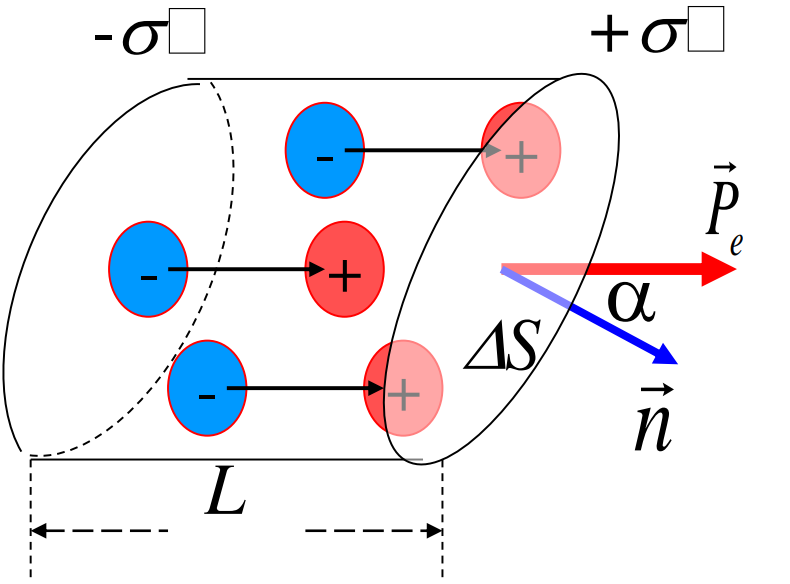
\includegraphics[width=0.5\textwidth]{ch03.png}
\end{figure}

Tách ra khối trụ xiên có

\begin{itemize}
  \item Đường sinh có chiều dài $L$, song song $\vec{E}$
  \item Hai đáy song song có diện tích $\Delta S$
  \item $+\sigma', -\sigma'$ là mật độ điện mặt mỗi đáy
  \item $\vec{n}$ là pháp tuyến của mặt tích điện dương
\end{itemize}

Coi khối trụ xiên như 1 lưỡng cực điện có 2 điện tích $+\sigma' \Delta S$ và $-\sigma' \Delta S$ cách nhau $L$.

\begin{equation*}
  P_e = \left| \vec{P}_e \right| = \frac{\sigma' \Delta S L}{\Delta S L \cos\alpha} = \frac{\sigma'}{\cos\alpha} 
  \Rightarrow \sigma' = P_e\cos\alpha = P_{en}
\end{equation*}

Mật độ điện mặt có giá trị bằng vector phân cực điện môi chiếu lên phương pháp tuyến.

\subsection{Câu 2}

Tính cường độ điện trường tổng hợp trong điện môi:

\begin{itemize}
  \item Xét điện trường đều $\vec{E}_0$ giữa 2 mp mang điện tích bằng nhau trái dấu
  \item Chất điện môi lấp đầy khoảng giữa
  \item Xảy ra hiện tượng phân cực điện môi, xuất hiện điện tích liên kết $\sigma'$
  \item Điện trường phụ $\vec{E}'$
\end{itemize}

Có $\vec{E} = \vec{E}_0 + \vec{E}' \Rightarrow E = E_0 - E'$

\begin{gather*}
  \begin{cases}
    E' = \frac{\sigma'}{\epsilon_0}\\
    \sigma' = P_{en} = \epsilon_0 \chi_e E
  \end{cases}
  \Rightarrow E' = \chi_e E \\
  E = E_0 - \chi_e E \Rightarrow E = \frac{E_0}{1+\chi_e} = \frac{E_0}{\epsilon}
\end{gather*}

Hiệu ứng áp điện:

\begin{itemize}
  \item Áp điện thuận: Khi nén hoặc kéo giãn một số tinh thể điện môi, xuất hiện điện tích trái dấu
  \item Áp điện nghịch: Khi đặt lên hai mặt của tinh thể một hiệu điện thế thì bị nẽn hoặc giãn
\end{itemize}